%\documentclass[pageno]{jpaper}
\documentclass[12pt]{report}

\usepackage[normalem]{ulem}
\usepackage{graphicx}
\usepackage{caption}
%\usepackage{subcaption}
\usepackage{amsmath}
\usepackage{amssymb}
\usepackage{color}
\usepackage{listings}
\usepackage{booktabs}
\usepackage{geometry}
\usepackage{fixltx2e}
\graphicspath{ {figures/} }
\geometry{margin=0.75in}
%\lstset{basicstyle=\footnotesize,frame=single}

\definecolor{dkgreen}{rgb}{0,0.6,0}
\definecolor{gray}{rgb}{0.5,0.5,0.5}
\definecolor{mauve}{rgb}{0.58,0,0.82}

\lstset{frame=none,
  language=bash,
  aboveskip=3mm,
  belowskip=3mm,
  showstringspaces=false,
  columns=flexible,
  basicstyle={\small\ttfamily},
  numbers=none,
  numberstyle=\tiny\color{gray},
  keywordstyle=\color{blue},
  commentstyle=\color{dkgreen},
  stringstyle=\color{mauve},
  breaklines=true,
  breakatwhitespace=true,
  tabsize=3
}



\newenvironment{blockquote}{%
	\par%
	\medskip
	\leftskip=2em\rightskip=2em%
	\ignorespaces}{%
	\par\medskip}
 
\begin{document}

\title{
    {Cryogenic Control Analysis and Optimization for Quantum Computation}\\
    {\small An infrastructure for analysis of classical control unit architectures for quantum computation}\\
}


\author{Adam Holmes}

\date{September 2016}



\maketitle

\chapter*{Framework Overview}
%\section*{Framework Overview}~\par
To perform quantum computation, classical control units will be located at one (or more) temperature level(s) of dilution refrigerator-based superconducting quantum computers. The question considered in this work is: what are the tradeoffs between targeting lower computation or lower memory usage within classical control units with differing hardware constraints located at different temperature levels? To this end, the parameters under consideration are:
\begin{itemize}
	\item Dilution Refrigerator Constraints, 
	\item Hardware Characteristics, and
	\item Benchmark Code Generation and Manipulation. 
\end{itemize}
\subsection*{Dilution Refrigerator Constraints}

The architecture of a dilution refrigerator being considered is a multi-stage cooling apparatus, using liquid nitrogen and liquid helium. Of interest right now are two characteristics: cooling capacity of temperature stages and latency of microwave links crossing these thermal boundaries. Using information from the specifications of a typical refrigerator (specifically the Oxford-Instruments TritonXL), these temperature levels and cooling capacities are shown in Table \ref{t2}.

\begin{table}[h!]
	\centering
    \begin{tabular}{|c|c|}
    \hline
    Temperature Stage (Kelvin) & Cooling Capacity (Watts) \\ \hline
    $20$ mK & $25$ $\mu$W \\ \hline
    $100$ mk & $1$ mW \\ \hline
    $4$K & $1.35$-$2$W \\
    \hline
    \end{tabular}
    \caption{Temperature Levels and Cooling Capacities}\label{t1}
\end{table}

These figures are approximate, and relate specifically to one realization of a dilution refrigerator, so are definitely subject to change. They differ somewhat from the estimates brought up in discussions, where we saw that the 20 mK level cooling capacity is approximately two orders of magnitude less than the cooling power available at the 4K temperature level. Further clarification will be sought to establish correct figures. 

Additionally, there is a range of latencies introduced in passing microwave links through temperature interfaces. These seem to vary between 1-10ns approximately, growing longer as the gap widens between the target temperatures of the stages being crossed.

\subsection*{Hardware Characteristics}

There are three primary types of hardware under consideration:
\begin{itemize}
	\item RSFQ: Rapid Single Flux Quantum
	\item RQL: Reciprocal Quantum Logic
	\item CryoCMOS: Cryogenic CMOS
\end{itemize}
Each of these is characterized by a different energy usage/logic gate relationship. these values are typically characterized similarly to Table \ref{t2}.
\begin{table}[h!]
	\centering
	\begin{tabular}{|c|c|}
	\hline
	Hardware Type & Energy Required Per Gate (Joules) \\ \hline
	RSFQ & $10^{-19}$ \\ \hline
	RQL & $10^{-19}$ \\ \hline
	CryoCMOS & $10^{-15}$ \\
	\hline
	\end{tabular}
	\caption{Hardware Types and Energy Consumed Per Gate}\label{t2}
\end{table}

These can be used directly to convert between computation and energy, and will be inserted into the model.

It is also important to consider power consumption of memory systems under these types of conditions. Here, we will analyze power usage of cryogenic CMOS memory devices, and consider implementations of cryogenic persistent memory systems. Persistent memory could potentially be useful in applications that rely upon a precomputed library of rotation decompositions, as memory may only need to be read only for long periods of computation. The qualification is that different applications often require different levels of precision in rotation decompositions, so these databases would potentially need to be changed between apps.

\subsection*{Program Code Generation and Manipulation}

The last set of variables being considered are those relating to the generation of instruction code for these quantum benchmarks. These techniques fall into several categories, specifically the relationship between the compilation flattening threshold and code caching behavior, and methods of compressing and decompressing modules. 


\chapter*{Roadmap}
The analysis will progress in stages. First an abstract model of a classical control unit as a cache is built, along with various methods for communicating program data to and from the cache. In this stage, program modules are extracted from full logical schedules which are compiled with the ScaffCC framework \cite{scaff}, and various cache compression techniques are explored for reducing the minimum required memory size of the control unit. Initial analysis will compare the effect of variable module compression techniques against the required computation introduced by performing the compression and decompression actions, which ultimately affects overall quantum program runtime. \par ~\par 
	The next stage is the construction of an energy budget cost model, which incorporates cooling capacity constraints of the different temperature interfaces of a dilution refrigerator with the effective energy usage per operation of different hardware materials. The cache model of classical control is expanded by introducing these new costs as constraints on computation, which affects the ability to perform module decompression and maintain the target temperature for a specified region. Techniques for optimizing module compression and decompression will be explored. Additionally, parameters describing latency caused by microwave links traversing thermal boundaries will be introduced as communication costs, which will be incorporated into the cost model.\par ~\par
	The following stage will begin to analyze the tradeoffs of different flattening thresholds for code modularization during compilation of quantum programs. Conceptually, flattening quantum benchmarks with a high gate count threshold will allow the compiler to be more efficient and reduce overall runtime, as more context is available during these optimizations. However this increases the size of each module, which increases the complexity and overhead of the caching mechanism. The interaction between these behaviors will be analyzed, and new techniques of both code modularization and module compression and decompression will be explored to optimize quantum program execution.\par ~\par 
		The ultimate goal of this analysis is to extract and quantify specific tradeoffs with system design choices involving control unit hardware, temperature level placement of control units, and memory sizes of control units. The aim is also to develop novel techniques for optimizing the transmission of large quantum programs through a control unit system, including optimized module compression and decompression methods for both control unit memory size reduction and communication bandwidth requirement reduction. 



\chapter*{Stage One: Cache Implementation and Initial Results}
\section*{Cache Model}~\par
	The initial phase of analysis is the construction of a model of classical control units as caches for quantum programs. Conceptually, quantum programs are compiled and scheduled with the ScaffCC framework which results in discretization of the programs into modules. Each of the modules compiled such that they self contained, and have no dependencies upon other modules with potential exceptions at module boundaries. The largest uncompressed module size provides a lower bound on the size of the cache memory.\par
	Simulations are performed on a per-program basis. The modules of each program are extracted, and unique binary codes are assigned to individual instructions, quantum register names, as well as module calls themselves. Once each module is converted to binary, each is compressed and decompressed across a series of different compression algorithms, and statistics regarding CPU usage and memory usage are collected with respect to each module. A program call stack is then simulated on control units of varying capacities (parameterized by number of containable modules), and total CPU usage required by decompression of modules is tracked. These statistics are then compared against the overall program runtime to determine significance of the decompression actions. Examples of these simulations are provided in (figure \ref{fig:ising}) and (figure \ref{fig:bwt}).\par 
	
\section*{Initial Results}
	Provided here are examples of the first stage statistics. The first set of plots depict the total CPU usage requirements for two different quantum programs, Ising Model and Binary Welded Tree. As can be seen, the CPU usage depends highly on the structure of the program module sizes.\par
\begin{figure}[h]
	\begin{minipage}{0.5\textwidth}
		\centering
		\includegraphics[width=\linewidth]{Figures/ising.png}
		\caption{Ising Model}
        \label{fig:ising}
	\end{minipage}\hfill
	\begin{minipage}{0.45\textwidth}
		\centering
        \includegraphics[width=1.1\linewidth]{Figures/bwt.png}
		\caption{Binary Welded Tree}
        \label{fig:bwt}
	\end{minipage}
\end{figure}

	The next analysis compares the CPU usage-padded runtimes against original program runtimes. Provided are two plots, the former (figure \ref{fig:full}) of the new program slowdowns due to decompressions, and the latter (figure \ref{fig:fullfocus}) a scaled view of the same plot. Slowdowns shown here are considerable, higher than 100x for many benchmarks. \par 
\begin{figure}[h]
	\begin{minipage}{0.5\textwidth}
		\centering
		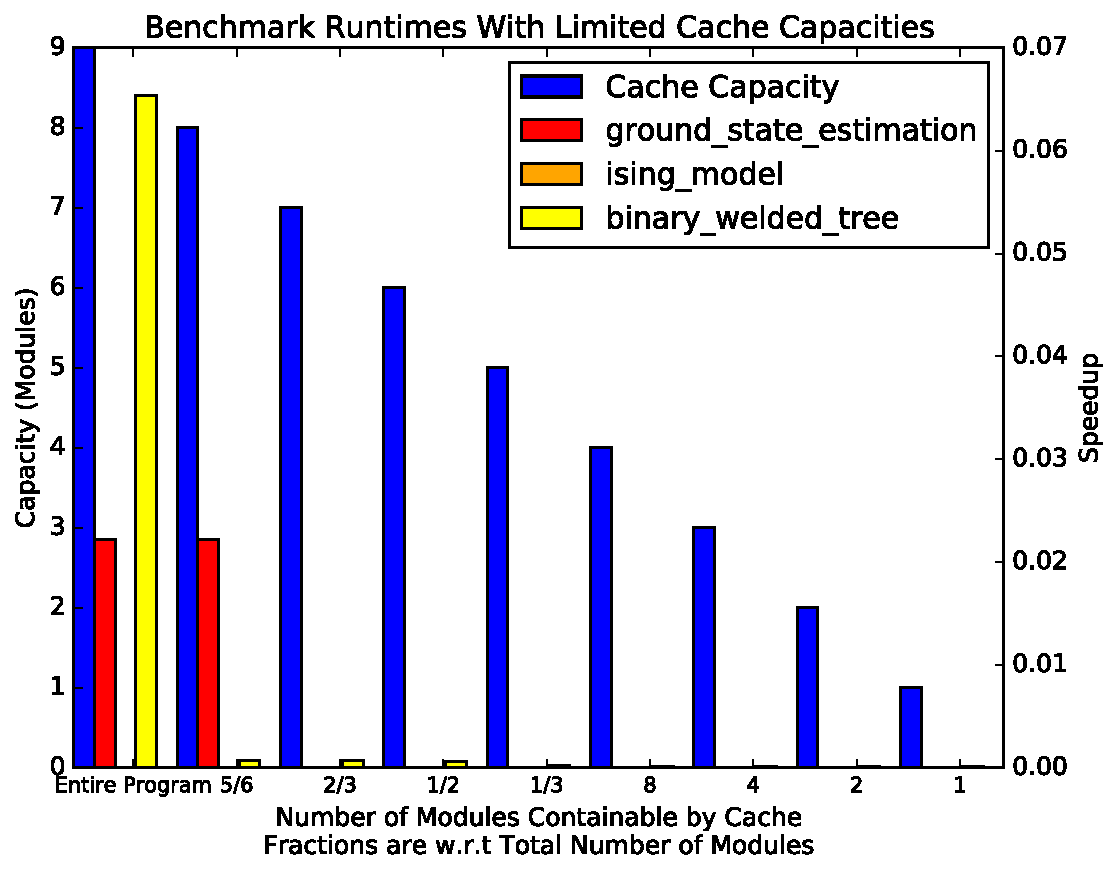
\includegraphics[width=\linewidth]{Figures/full.pdf}
		\caption{New Program Runtimes with Decompressions}
        \label{fig:full}
	\end{minipage}\hfill
	\begin{minipage}{0.45\textwidth}
		\centering
        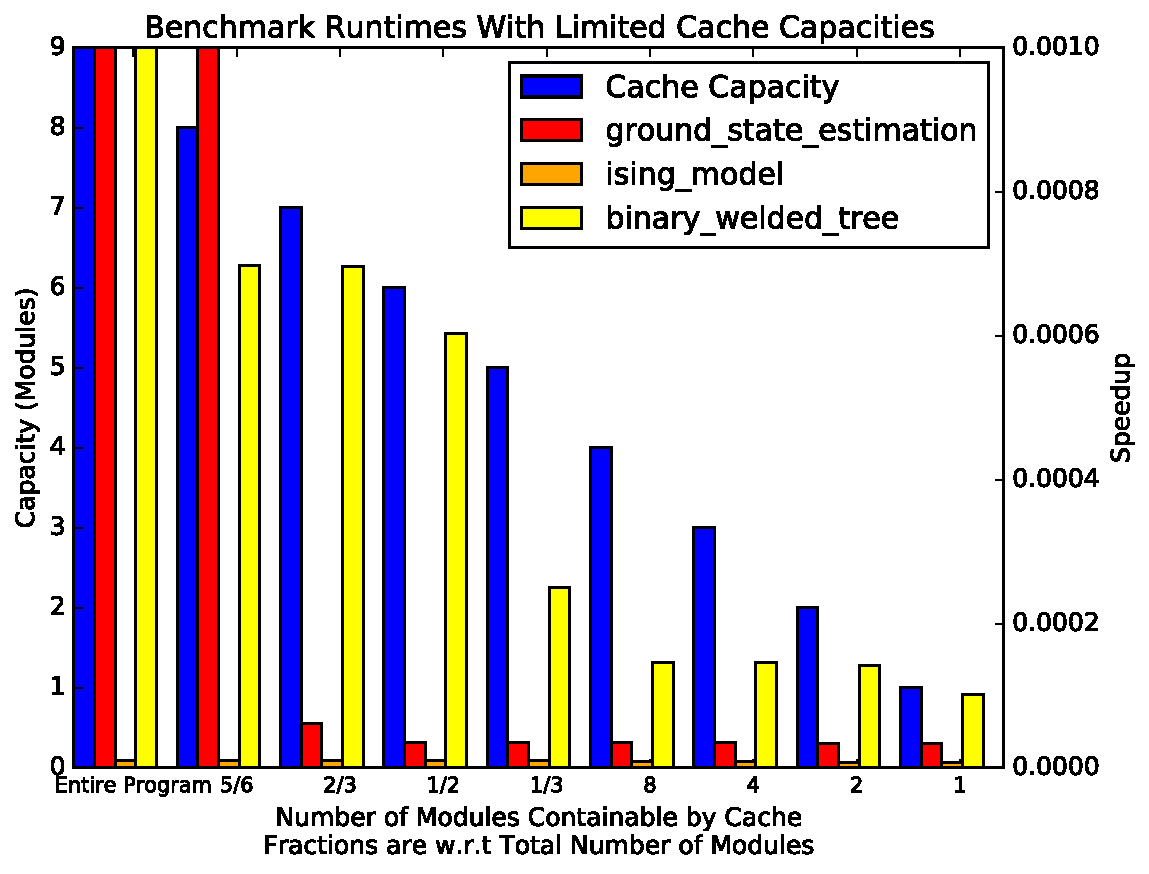
\includegraphics[width=1.1\linewidth]{Figures/fullfocused.pdf}
		\caption{Scaled Depiction of New Program Runtimes}
        \label{fig:fullfocus}
	\end{minipage}
\end{figure}

This initial analysis is intended to motivate the idea that restricting the memory sizes of control units has a dramatic effect on the runtimes of quantum programs, with dependence upon the internal structure of the program and distribution of module sizes.


%\chapter*{Stage Two: Energy Budget Implementation and Results}
%\input{chapters/stage_two}
%
%\chapter*{Stage Three: Compiler Configuration and Code Decompression Technique Exploration and Results}
%\input{chapters/stage_three}


\bibliography{references}
\bibliographystyle{IEEEtranS}

\end{document}
